\documentclass{article}
\usepackage{hyperref}
\usepackage{listings}
\usepackage{graphicx}
\usepackage[margin=1in]{geometry}
\usepackage{titlesec}
\usepackage{enumitem}
\usepackage{amsmath}
\usepackage{xcolor}
\usepackage{biblatex}
\addbibresource{references.bib}
\titleformat{\section}{\normalfont\Large\bfseries}{\thesection}{1em}{}
\titleformat{\subsection}{\normalfont\large\bfseries}{\thesubsection}{1em}{}

\graphicspath{{images/}}

\title{Toward Decentralized Trust and Verifiable Content on the Web}
\author{
  Jason Grey\\
  \texttt{jason@jason-grey.com}
}
\date{}

\begin{document}

\maketitle

\begin{abstract}
We propose a decentralized, standards-aligned framework for embedding cryptographic trust directly into HTML content. Using a new \texttt{<signed-section>} element, content creators and publishing platforms can sign semantically meaningful regions of web pages and include identity-linked metadata in-band. Signatures are validated using public key infrastructure (PKI) such as DIDs \cite{DIDSpec}, and can be enhanced with third-party endorsements submitted to optional, federated trust directories. We define a canonicalization method for content normalization and show how browsers and CMS systems can support user-configured web-of-trust policies for live content validation. The scheme is fully implemented: five independent language libraries, a reference trust directory, a browser verifier, and static-site and CMS signers reproduce a shared conformance suite and a complete end-to-end test vector byte-for-byte, and we report the specific text-normalization hazards this cross-implementation discipline surfaced and resolved. Unlike blockchain-based or DRM-centric systems, our approach is lightweight, browser-compatible, and web-native---designed to scale across publishing workflows, civic media, and knowledge networks.
\end{abstract}

\section{Introduction}

The web lacks a standardized mechanism for proving who wrote or who was first to publish a given piece of content. TLS certifies the domain, but not the author. As AI-generated and republished material becomes ubiquitous, users face increasing difficulty determining what content is trustworthy. Existing methods like digital signatures (e.g., DKIM \cite{DKIM}, PGP \cite{PGP}) and content fingerprinting (e.g., ISCC \cite{ISCC}) offer pieces of the solution but do not integrate cleanly with web-native publishing workflows or browser verification.

We present a system for decentralized content authenticity, authorship claim, and endorsement that aligns with the hypertext ethos: structured, inspectable, and layered. We define a method for authors to sign content blocks in HTML, supported by canonicalization rules and cryptographic integrity checks, along with an endorsement and discovery model via public trust directories.

\section{System Architecture}

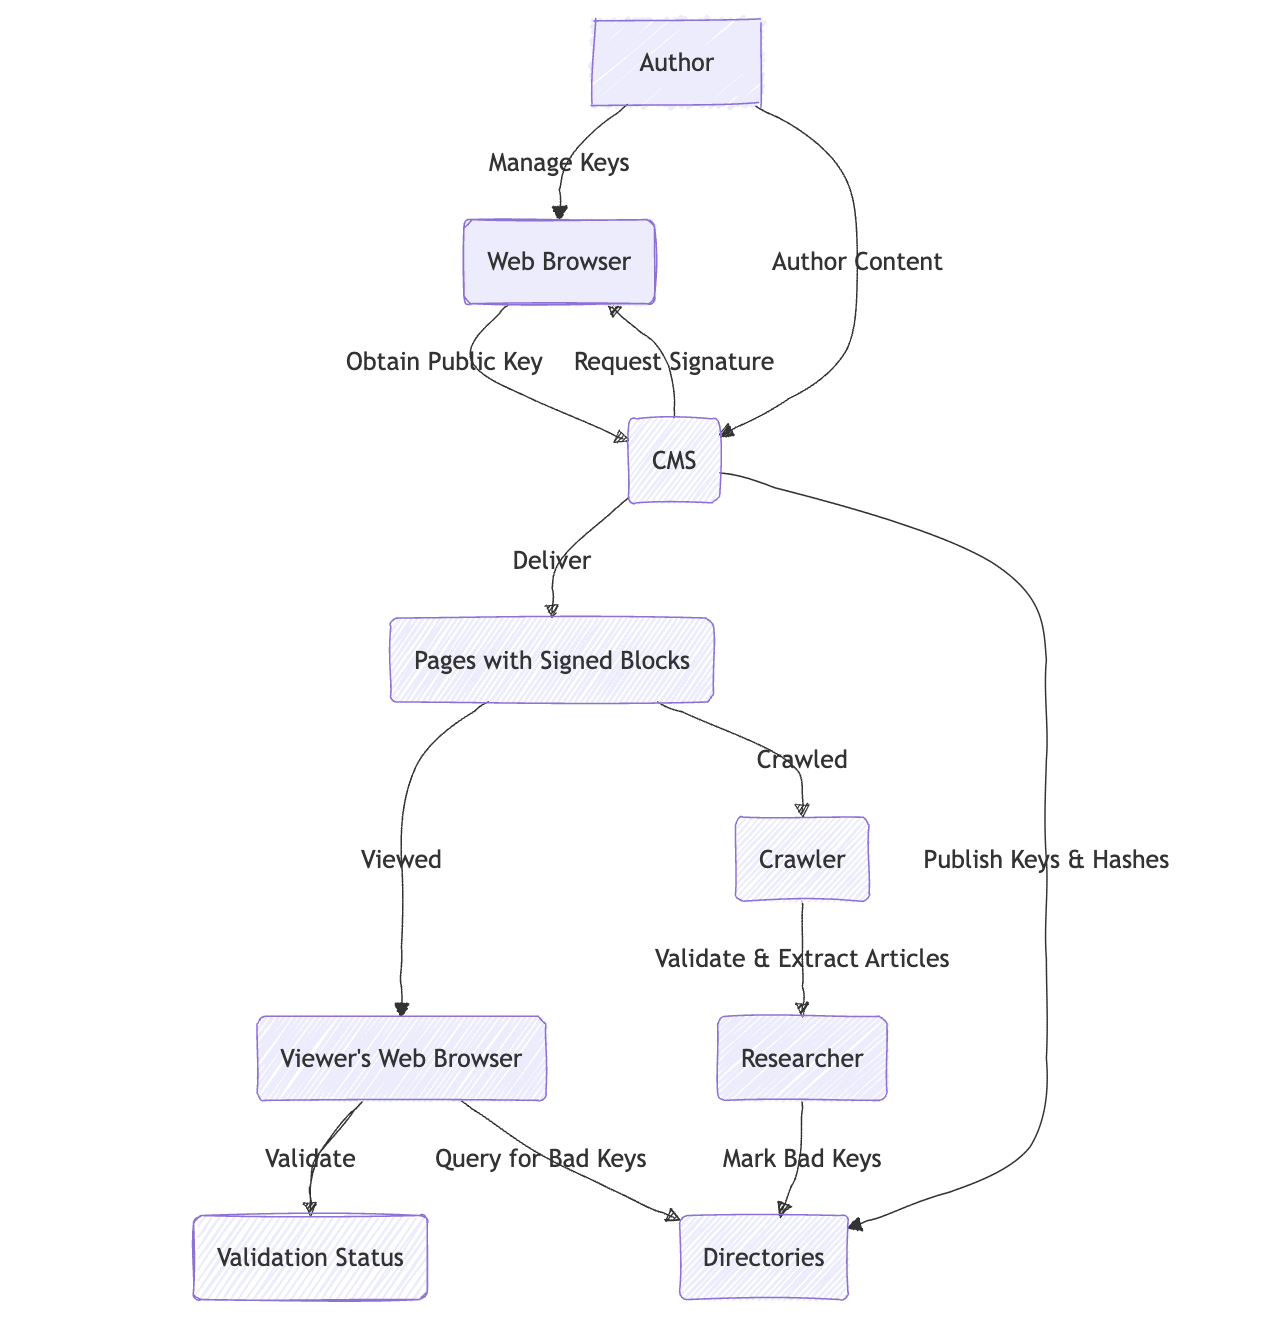
\includegraphics[width=\textwidth]{architecture1}

\subsection{Signed HTML Blocks}
A new tag, \texttt{<signed-section>}, encapsulates a signed region of a page. This tag carries the cryptographic signature and its supporting metadata as attributes, and its inner content includes the signed content itself and any claims expressed as \texttt{<meta>} elements.

\begin{lstlisting}[language=HTML, basicstyle=\ttfamily\footnotesize]
<signed-section keyid="did:web:author.example"
    signature="3q2+7w8NslfJ..."
    content-hash="sha256:RAyBCvKT..."
    algorithm="ed25519">
  <meta name="author" content="Alice Example">
  <meta name="signed-at" content="2025-05-01T10:30:00Z">
  <meta name="claim:License" content="CC-BY-4.0">
  <article>
    <h1>Verifiable Web Content</h1>
    <p>Content should be provable...</p>
  </article>
</signed-section>
\end{lstlisting}

\paragraph{Required attributes.} \texttt{keyid} (identifies the signer, resolvable per \S2.2), \texttt{signature} (the cryptographic signature, encoded per the hash encoding rules below), \texttt{content-hash} (hash of the canonicalized content, prefixed with the hash algorithm, e.g. \texttt{sha256:\ldots}), and \texttt{algorithm} (a registered signature-algorithm identifier: \texttt{ed25519} is mandatory to implement, with \texttt{ecdsa-p256}, \texttt{ecdsa-p384}, \texttt{rsa-pss-sha256}, and \texttt{rsa-pkcs1-sha256} also registered).

\paragraph{Hash and signature encoding (open feedback).} Hashes and signatures in this revision are encoded as unpadded Base64, which is shorter than hexadecimal by roughly one-third. We invite community feedback on whether hexadecimal (widespread in tooling such as git and TLS), Base32 (case-insensitive and easier to transcribe by hand), or another encoding would be preferable for broader ecosystem alignment.\footnote{Or Ecoji, anyone? A 32-byte SHA-256 digest encodes to 26 emoji characters via the Ecoji base-1024 alphabet, producing a delightfully unreadable \texttt{content-hash="sha256:<26 emoji from the Ecoji alphabet>"}. It is, alas, \textit{longer} in wire bytes because each emoji occupies four UTF-8 bytes, so we have not adopted it. But we thought you should know it exists.}

\paragraph{Canonical signing payload.} The signature is computed over a deterministic binding string:
\begin{lstlisting}[basicstyle=\ttfamily\footnotesize]
{content-hash}:{claims-hash}:{domain}:{signed-at}
\end{lstlisting}
where \texttt{content-hash} is the hash of the canonicalized content, \texttt{claims-hash} is the hash of the canonical serialization of all inner \texttt{<meta>} claim elements (ordered lexically by name), \texttt{domain} is the origin where the content is authoritatively published, and \texttt{signed-at} is the RFC 3339 date-time (in UTC) from the corresponding \texttt{<meta>} tag. The signer's identity is not included in the binding because it is implicit in the keyid resolution step: any attempt to claim a signature under a different identity would resolve to a different public key and fail verification.

Domain binding intentionally ties a signature to a specific publication origin, preventing unauthorized republication of signed content with the original signature preserved. Legitimate republication is supported through a separate mechanism: a republisher MAY wrap the signed content in their own outer \texttt{<signed-section>} that references the original via a canonical-URL metadata field, preserving the integrity of the original while adding an attribution chain. (This wrapped-signing mechanism is defined in future work.)

\paragraph{Canonical content extraction.} The hash over which the signature is computed is taken from the \textit{text content} of the signed region after the extraction and normalization process defined in \S\ref{sec:canon}. Element markup---the start and end tags themselves---is not covered by the hash. A small, fixed set of \textit{signed semantic attributes} \emph{is} covered: \texttt{href}, \texttt{src}, \texttt{alt}, and \texttt{aria-label}. These carry reader-visible meaning (link and image destinations, and the accessible text screen-reader users consume) that a text-only hash would otherwise leave malleable; binding them closes the in-region link-swap and image-swap vectors while stopping well short of full structural signing.

This design deliberately accepts certain semantic gaps at the protocol layer: an adversary in possession of signed text MAY rewrap it in misleading block elements, alter link destinations \emph{outside} the signed region, or surround it with additional media, all without invalidating the cryptographic signature. We consider these acceptable at the protocol layer because the HTMLTrust system addresses them through a higher, social layer: signatures are domain-bound (see the canonical signing payload above), so a reader encountering signed content at an unexpected origin is immediately alerted by the signature check itself, and crawlers and researchers (\S2.4) can trace signed content back to its canonical origin through the trust directory, flagging imposter copies and content that has been altered outside its original publication site. Cryptographic verification ensures \textit{the words are genuine and published where they claim to be}; the research and reputation ecosystem catches the remaining semantic attacks, such as altered surrounding context or link-swap on mirrored pages. The layered design keeps cryptographic verification simple, fast, and portable across implementations while delegating semantic-integrity detection to the research path, where it can evolve over time without breaking existing signatures.

\paragraph{Open design question: expanding attribute coverage.} This revision commits to the four attributes above; \texttt{href} in particular closes the in-region link-swap phishing vector that domain-binding and researcher traceability cannot fully address on their own. The remaining open question is \textit{how far} to extend the list---candidates include \texttt{title}, \texttt{cite}, and image dimension attributes---without drifting toward the full-structural signing that made XML Digital Signatures operationally unusable across implementations. Each addition widens the canonicalization surface that must remain byte-identical across every implementation (\S\ref{sec:results}), so the list is deliberately grown slowly and only for attributes with clear reader-visible semantics. We invite community feedback on this trade-off.

\subsection{Identity and Key Resolution}
The \texttt{keyid} attribute identifies the signer but is deliberately pluggable: implementations MUST accept multiple resolution methods and SHOULD treat none as canonical. Acceptable forms include:

\begin{itemize}
  \item \textbf{Decentralized Identifiers (DIDs)}: e.g., \texttt{did:web:author.example}, which resolves via a well-known DID document hosted at the author's origin \cite{DIDSpec}. This places no dependency on any third party.
  \item \textbf{Direct URL to a public key}: e.g., \texttt{https://author.example/key.json}, fetched directly from the author's origin. Simple to host as a static file without additional tooling.
  \item \textbf{Trust directory reference}: e.g., \texttt{https://directory.example/keys/abc123}, where a federated trust directory serves as a convenience key registry. This is particularly useful for less-technical authors who prefer a ``signup'' workflow to self-hosted identity publication.
\end{itemize}

None of these methods places a privileged entity at the center of the web-of-trust: authors freely choose a resolution mechanism, and verifiers freely choose which methods they accept. The \texttt{keyid} is opaque to the signature protocol; only the resolved public key matters for cryptographic verification, which is a local operation in the user agent and never requires contacting a directory.

\subsection{Canonicalization}
\label{sec:canon}
The security of the scheme rests entirely on \emph{byte-identical} canonicalization: a signer and any independent verifier must derive exactly the same UTF-8 byte string from the same signed region, or the signature fails. Canonicalization operates on the \textit{text content} of the signed subtree---element start and end tags contribute no bytes---plus a small, fixed set of signed semantic attributes. For each text node, in order: (1) Unicode NFKC normalization; (2) removal of a fixed set of invisible and bidirectional formatting characters, while preserving the zero-width non-joiner and joiner, which are semantic in Persian, Indic scripts, and emoji sequences; (3) mapping of all Unicode whitespace to U+0020, with runs collapsed and each block trimmed; (4) normalization of typographic punctuation (curly quotes, dashes, ellipses) to ASCII. Block-level elements emit a single line-feed boundary. HTML character references are decoded per the HTML Living Standard parse model---the full named-reference set, matched case-sensitively, plus numeric references with the standard replacement rules---before normalization. Four signed semantic attributes---\texttt{href}, \texttt{src}, \texttt{alt}, and \texttt{aria-label}---are emitted as explicit records; URL-valued attributes are serialized with the WHATWG URL serializer, so that host case, default ports, dot-segments, and internationalized (IDNA/punycode) hosts canonicalize identically across implementations. Claim \texttt{<meta>} elements are excluded from the content and hashed separately, sorted by the UTF-8 byte order of their normalized names.

Getting this layer wrong is the dominant failure mode for cross-implementation signing systems; the operational fragility of XML Digital Signatures \cite{XMLDSIG} across implementations is the canonical cautionary example. We therefore treat byte-level interoperability as a first-class deliverable rather than an implementation detail. The normative rules are pinned by a shared conformance suite and by published end-to-end test vectors---a fixed key, a fixed HTML fixture, and the exact canonical bytes, content and claims hashes, signing payload, and signature---that every implementation reproduces in continuous integration. Section~\ref{sec:results} reports the cross-language interoperability results and the specific normalization hazards this discipline surfaced.

\subsection{Trust Directory (Optional)}
Signed content MAY be submitted to one or more trust directories. A directory MAY perform any of the following roles, and implementations MAY specialize in a subset:
\begin{itemize}
  \item Indexes content hashes and associated signers for discovery.
  \item Stores and serves third-party endorsements.
  \item Supports key resolution and optional revocation.
  \item Acts as a convenience key registry and ``signup'' provider for authors who prefer not to self-host identity documents.
\end{itemize}

Directories are federated: multiple directories MAY coexist, and user agents MAY query any subset of them according to user policy. No directory is privileged by the protocol, and verification of a signature never requires contacting a directory---only key resolution (when the chosen \texttt{keyid} form points at a directory) and optional endorsement lookup do.

\subsection{Endorsements}
Third parties (publishers, experts, other users) MAY issue signed JSON endorsements of specific content hashes. An endorsement is a standalone signed artifact that attests the endorser's opinion about a specific piece of signed content at a specific moment in time:

\begin{lstlisting}[basicstyle=\ttfamily\footnotesize]
{
  "endorser": "did:web:publisher.org",
  "endorsement": "sha256:XYZ...",
  "algorithm": "ed25519",
  "timestamp": "2025-05-01T00:00:00Z",
  "signature": "BASE64_SIG"
}
\end{lstlisting}

The endorsement signature is computed over the RFC 8785 JSON Canonicalization Scheme (JCS) serialization of the object with the \texttt{signature} field omitted, so that any verifier reconstructs identical signed bytes regardless of key ordering or JSON formatting. The endorsed content hash carries the same \texttt{sha256:} algorithm prefix and unpadded-Base64 encoding as content hashes, and the timestamp is an RFC 3339 date-time in UTC.

Endorsements target specific pieces of content, not signers. Ongoing or collective trust of a signer is expressed via that signer's reputation in one or more trust directories (see \S2.4), not via persistent signer-level endorsement artifacts. This separation keeps endorsement semantics clean: a content endorsement is a point-in-time attestation about a specific artifact, while directory reputation reflects an ongoing curatorial opinion about a signer.

Endorsements are stored and served by trust directories, which index them by content hash. A verifier seeking endorsements for a given piece of content queries one or more directories and retrieves any endorsements on file. Endorsements MUST be verified cryptographically by the verifier using the endorser's public key (itself subject to the same keyid resolution methods as content signatures) before being trusted. An unverified endorsement MUST NOT contribute to any trust decision.

\section{Browser and CMS Integration}

\subsection{Browser Behavior}
User agents perform verification in two distinct layers:

\begin{itemize}
  \item \textbf{Cryptographic verification (local)}: The user agent canonicalizes the signed content, computes its hash, compares it against the embedded \texttt{content-hash}, resolves the \texttt{keyid} to a public key, and validates the signature. This is a local operation, performed in the user agent with no network calls beyond the key resolution step, and produces a deterministic yes/no result.
  \item \textbf{Trust decision (client policy)}: Given a cryptographically valid signature, the user agent applies the current user's trust policy to decide how to present the content. This may consider the author's identity against a personal trust list, endorsements from trusted third parties, optional reputation queries to one or more trust directories, and local or cached revocation state. The outcome is user- and context-specific and is never determined by a remote authority.
\end{itemize}

Trust configuration is client-side. Trust policies MAY draw on any combination of inputs, including personal trust lists of keyids, domain-level trust for origins, transitive trust via endorsements from designated parties, and reputation scores produced by user-selected trust directories. A trust directory MAY compute scores using its own curated trust graph, which subscribing users inherit without maintaining their own graph; this federates the burden of trust graph maintenance to directory operators whom users choose to trust at a higher level.

User interfaces SHOULD present the trust outcome as a graduated score or ranking rather than a binary verdict, and SHOULD distinguish the two layers visually: a signature either verifies cryptographically or it does not, but trust is a matter of degree. A score-based indicator (e.g., red below a low threshold, green above a high threshold, yellow in between) with hover or detail views exposing the underlying rationale (which inputs contributed, which directories were consulted, which endorsements applied) allows users to distinguish cryptographic certainty from social trust, and to understand why a given piece of content earned the indicator they see.

\subsection{CMS Workflows}
Content management systems (or social media platforms, etc.) generate:
\begin{itemize}
  \item Canonicalized content blocks.
  \item Embedded signatures from author keys.
  \item Optional submissions to trust directories.
\end{itemize}

\section{Related Work}

HTMLTrust draws on prior art across three categories: per-resource transport integrity, identity and credential infrastructure, and community efforts addressing content credibility on the open web.

\paragraph{Per-resource transport integrity.} DomainKeys Identified Mail (DKIM) \cite{DKIM} attests to message integrity and signer authority at the SMTP layer through DNS-published keys; its operational template informs HTMLTrust's separation of cryptographic verification from policy-driven trust decision. JSON Web Signature \cite{JWS} is the widely deployed envelope for signed JSON; HTMLTrust endorsements instead sign the RFC 8785 canonical serialization of a directly-inspectable JSON object (its \texttt{signature} field omitted), avoiding JWS's base64url-wrapped payload. Signed HTTP Exchanges \cite{OriginSigned} certify a complete HTTP response from a specific origin, but operate at response granularity and have not been adopted outside Google's AMP infrastructure. Subresource Integrity \cite{SRI} provides byte-level integrity for fetched subresources, with no attestation of authorship and no coverage of per-region content within an already-loaded document. XML Digital Signatures \cite{XMLDSIG} attempted full structural signing of XML; its operational fragility across implementations is a cautionary precedent that motivates HTMLTrust's deliberately narrow semantic-subset signing.

\paragraph{Identity and credential infrastructure.} The W3C Decentralized Identifiers specification \cite{DIDSpec} and the W3C Verifiable Credentials Data Model \cite{VCDataModel} provide the identity and attestation primitives that HTMLTrust uses for key resolution and endorsement formatting. Both are normative dependencies rather than competitors. The Coalition for Content Provenance and Authenticity (C2PA) \cite{C2PA} addresses provenance for image, video, and document assets through metadata sidecars; HTMLTrust extends an analogous goal to in-document HTML text regions, in band rather than via sidecars.

\paragraph{Community efforts on web credibility.} Several active W3C Community Groups address adjacent or overlapping concerns. The Credible Web Community Group \cite{CredibleWeb} has produced the \textit{Credibility Signals} catalog and hosts research on reputation graphs, credibility scoring, and originator-profile mechanisms; the Originator Profile initiative \cite{OriginatorProfile} presented to that group in August 2024 is an independent author-attestation effort with origins in Japanese news media. The Decentralized Fact-checking and Provenance Organization Community Group (DeFacto) \cite{DeFacto} researches decentralized provenance and fact-checking specifications for text-based content, an architectural neighbor of the trust directory and endorsement components of this work. The AI Content Disclosure Community Group \cite{AIContentDisclosure} is defining structured syntax for declaring AI-authored content under emerging regulatory regimes including the EU AI Act; HTMLTrust's \texttt{claim:} namespace metadata is intended to compose cleanly with such disclosure markup when carried inside a signed section. The Credentials Community Group \cite{CredentialsCG} is the originating community for both DID Core and the Verifiable Credentials Data Model, and continues to steward the cryptosuite work on which HTMLTrust depends. The Anti-Fraud Community Group \cite{AntiFraudCG} addresses web-platform mitigations for fraudulent content delivery, an adjacent threat surface to the author-impersonation problem this work addresses.

HTMLTrust occupies a position none of these efforts directly fills: a cryptographic, browser-verifiable attestation of authorship for arbitrary HTML text regions, carried in band and verifiable without contacting any privileged authority. It is designed to compose with the credibility-signals and disclosure-metadata work above as inputs to the client-side trust-scoring layer described in \S3.

\section{Implementation and Results}
\label{sec:results}

The design above is fully implemented. The wire format is specified in an IETF Internet-Draft, and the system is realized as: five independent canonicalization libraries (JavaScript, Go, Python, Rust, and PHP); a reference federated trust-directory server with an OpenAPI description; a browser verifier available both as an extension and as a standalone client library; a Hugo static-site signer and a WordPress publishing plugin; and an end-to-end test harness that exercises the full signer-to-verifier path.

\paragraph{Cross-implementation interoperability.} Because the security of the scheme depends on byte-identical canonicalization (\S\ref{sec:canon}), we treat interoperability as a measured result rather than an assumption. A shared conformance suite (54 fixtures at the time of writing, including negative fixtures that assert a canonicalizer \textit{must} reject an input) is executed against every language binding in continuous integration, alongside a complete end-to-end test vector---a fixed Ed25519 key, a fixed HTML fixture, and the exact canonical bytes, content and claims hashes, signing payload, and signature---that each signer and verifier reproduces. All five implementations agree byte-for-byte across the suite.

\paragraph{Interoperability on the real web.} Passing a synthetic suite is necessary but not sufficient, so we ran the five canonicalizers over 5{,}146 real news-article regions deterministically sampled from Common Crawl's news corpus, inside a single pinned multi-language container. The synthetic agreement did not survive contact with real HTML. Byte-identical output across all five implementations held on only 20\% of real pages, and the study surfaced two show-stopper defects the fixtures could not: three of the five bindings rejected the opaque URL schemes (\texttt{mailto:}, \texttt{tel:}, \texttt{javascript:}, \texttt{data:}) that appear on over half of real pages, and the PHP binding's relative-reference resolver silently truncated paths on fragment-only links. Fixing both raised those bindings' success rate from roughly 46\% to 99\% and lifted all-implementations agreement to 31\%, but no further: the residual disagreement is dominated by five independent re-implementations of the URL serializer that do not byte-match a true WHATWG serializer on real URLs, and by the regex-versus-real-parser differential noted below (the two bindings that use a genuine WHATWG serializer and a real HTML parser still agree only 76\% of the time). Separately, re-serializing a page through a \textit{different} HTML5 parser---the kind of transformation a content-management pipeline routinely performs---preserved the canonical hash on roughly 88\% of pages, a measurable false-negative rate. We take this as the central open engineering result of the project: byte-identical canonicalization is solved for clean inputs and unsolved for the live web, and closing the gap requires one shared URL-and-parser implementation rather than several conformant-looking ports. The measurement harness and full results are released alongside the implementation.

\paragraph{Normalization hazards surfaced.} Reaching that agreement was not automatic; the conformance discipline exposed a series of text-normalization hazards that had silently diverged across independent implementations, each of which could yield the same signature verifying against different rendered content. We report them as a contribution in their own right, because they are the concrete landmines any cross-implementation HTML-signing effort will encounter:
\begin{itemize}
  \item \textbf{URL serialization.} A single \texttt{href} could canonicalize to as many as five different strings depending on host case, explicit default ports, dot-segment resolution, and internationalized-domain handling. We resolve this by mandating the WHATWG URL serializer (punycode hosts, resolved dot-segments, preserved query and fragment) in every binding.
  \item \textbf{Character references.} Bindings that decoded only a handful of common HTML entities diverged from those using a full parser on ordinary content such as \texttt{\&eacute;}. We require the full HTML5 named set, matched case-sensitively, plus the standard numeric rules.
  \item \textbf{Quotation-mark classing.} The single low-9 quotation mark (U+201A) had been mapped to a double quote across implementations, contradicting its Unicode single-quote semantics; German, Polish, and Czech text hashed inconsistently against any independent implementation built from the specification.
  \item \textbf{Claim ordering.} Sorting claim names by UTF-16 code units rather than UTF-8 bytes inverted the order of astral-plane versus high-BMP names, producing divergent claims hashes.
  \item \textbf{Excluded subtrees.} \texttt{<template>} and \texttt{<iframe>} content leaked into the canonical bytes in some bindings, allowing never-rendered markup to contribute signed content.
\end{itemize}
Each hazard is now pinned by a dedicated conformance fixture, so a regression is caught mechanically rather than discovered as a field interoperability failure.

\paragraph{Limitations.} Several bindings tokenize HTML with regular expressions rather than a full HTML parser; this is adequate for well-formed content but leaves a parser-differential risk on adversarial or malformed input, so trust-gating verifiers are required to use a real HTML parser. Whitespace inside \texttt{<pre>} is not byte-bound in this revision, a deliberate deferral until byte-identical per-element preservation across independent parsers is demonstrable. The client-side reputation layer is specified but its Sybil-resistance is not yet empirically evaluated. Finally, native \texttt{<signed-section>} support requires a multi-engine commitment from browser vendors; absent that, adoption depends on a crawl-time verifier at a search or answer engine---a DKIM-style bootstrap that does not require browser changes but that we have not yet measured at scale.

\section{Future Work}

Concrete next steps, in rough priority: (1) a crawl-time verifier deployed at a search or AI-answer platform and measured on a real content corpus, both to establish an adoption path independent of browser support and to quantify false-positive and false-negative rates in the wild; (2) a normative definition of wrapper re-signing (a \texttt{claim:CanonicalURL} envelope) so that legitimate republication carries an attribution chain rather than a broken signature; (3) an empirical Sybil-resistance analysis of the endorsement and directory-reputation layer; (4) a formal proposal for native \texttt{<signed-section>} support to the relevant browser-standards bodies; and (5) carefully scoped expansion of the signed-attribute set, each addition gated on demonstrated byte-identical support across all implementations.

\section{Conclusion}

This work introduces a practical, decentralized system for content authenticity on the web---one that is inspectable, implementable, and federated. It aligns with the Hypertext community's interest in authorship, provenance, and semantic structure while responding to misinformation and civic trust concerns.

By rooting trust in content itself and enabling configurable trust graphs, we reinforce the open web as a decentralized medium for human knowledge.

\printbibliography

\end{document}
